\section{Method}

\begin{figure*}[h!]
	\centering
	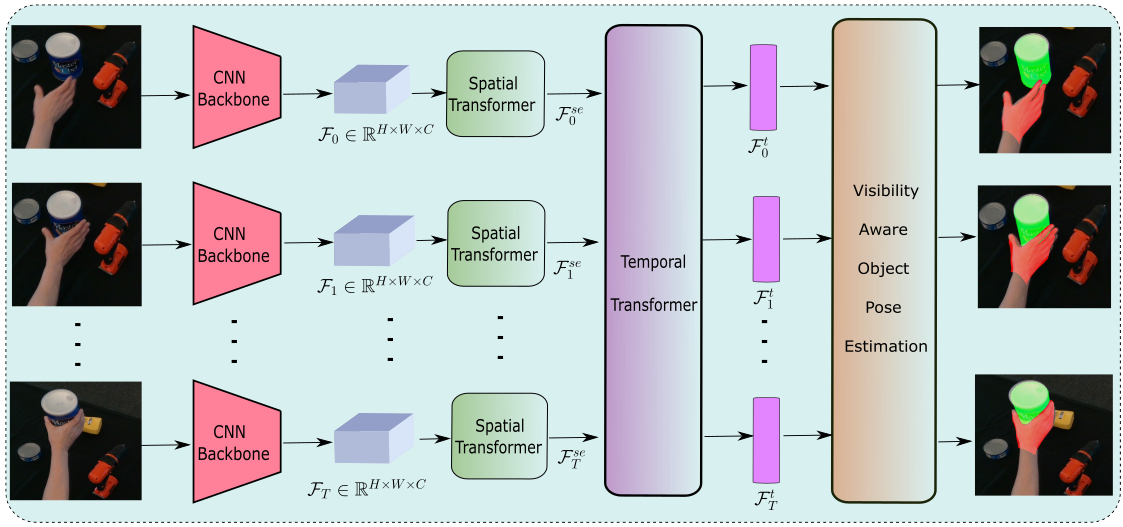
\includegraphics[width=0.98\linewidth]{figs/overview}
	\caption{Overview of the proposed framework for in-hand object pose tracking. Our approach leverages transformers to capture both spatial relationships within individual frames and temporal dependencies across image sequences, enabling robust frame-wise object pose estimation. To address challenges posed by heavy occlusion or motion blur, a visibility-aware module integrates temporally-aware features and aggregates pose information from neighboring frames. This allows the model to maintain accurate pose estimates even in difficult scenarios where direct visual cues are limited or absent.}
	\label{fig:overview}
\end{figure*}

The overview structure of our framework is illustrated in Figure \ref{fig:overview}. Given a sequence of RGB images $\mathcal{V} = \lbrace I_t \rbrace_{t=1}^{T}$, where $T$ represents the total number of frames, the objective is to estimate the object's 6D pose $\mathbf{P}_t = (\mathbf{R}_t, \mathbf{t}_t)$ for each frame $I_t$. This pose consists of the rotation matrix $\mathbf{R}_t$ and the translation vector $\mathbf{t}_t$, which describe the rigid transformation of the object from its coordinate system to the camera coordinate system. We assume that a 3D model of the object is available, and its coordinate system is defined within the 3D space of the model. The framework first utilizes a CNN backbone to extract spatial features \( \mathcal{F}_t \) from each frame. These features are then enhanced by a spatial transformer $\mathcal{M}_{s}$, which captures non-local dependencies within each frame to improve the modeling of complex hand-object interactions. The spatial transformer encoder produces contextually enriched features \( \mathcal{F}^s_t \), which are further processed by a temporal transformer $\mathcal{M}_{s}$ that models temporal relationships across frames. The temporal transformer outputs latent vectors \( \mathcal{F}^t_t \), which are passed through an MLP to predict the object's pose \( \hat{\mathbf{P}}_t \) for each frame. Additionally, a visibility-aware module $\mathcal{M}_{va}$ predicts the object's visibility score \( v_t \) for each frame, dynamically adjusting pose predictions based on occlusion levels. This module aggregates pose information from visible frames to support pose estimation in occluded frames using a cross-attention mechanism, ensuring robust performance under heavy occlusions and rapid motion.

\subsection{Spatial-Temporal Transformer}

\subsubsection{CNN Backbone}

Inspired by the hybrid model proposed by \cite{carion2020end}, our method begins by leveraging a truncated FPN \cite{lin2017feature} with ResNet50 \cite{he2016deep} to extract the initial in-hand object features $\mathcal{F}_t \in \mathbb{R}^{H \times W \times C}$ for each frame $I_t$. While CNNs, through their convolutional kernels, are effective at capturing local two-dimensional structures, they struggle with occlusions where local details are obscured or distorted. To mitigate this, we incorporate a transformer \cite{vaswani2017attention}, which is adept at handling non-local relationships and dependencies. The feature maps $\mathcal{F}_t$ are subsequently processed by a spatial transformer, which captures non-local dependencies within each frame, enhancing the network's ability to model complex interactions between the object and the hand.

\subsubsection{Spatial Transformer}

The spatial transformer encoder processes a sequence as input. To facilitate this, we flatten the spatial dimensions of the hand feature, resulting in $HW$ vectors, each with length $C$. These vectors, referred to as tokens, are then fed through multiple layers of multi-head self-attention and feed-forward networks (FFN). Since each transformer layer is permutation-invariant, we incorporate 2D positional embeddings into each token to provide spatial location information. The output feature $\mathcal{F}^s_t \in \mathbb{R}^{H \times W \times C}$ from the transformer encoder enhances the original feature $\mathcal{F}_t$ by capturing non-local interactions among all tokens. This enhanced feature $\mathcal{F}^s_t$ is expected to contain rich contextual information about the in-hand object, including the locations of object keypoints. We follow previous works \cite{oberweger2018making, tekin2018real, rad2017bb8} use the eight corners of the 3D bounding box of the object as the keypoints. As an intermediate supervision step, we regress a heatmap of object keypoint joints $\hat{\mathcal{H}}_t$ from $\mathcal{F}^s_t$, which provides the predicted locations of $N_j = 8$ keypoints as $\hat{\mathcal{K}} \in \mathbb{R}^{8 \times 2}$.

The spatial transformer decoder takes a learnable query vector $\mathbf{Q} \in \mathbb{R}^C$ as input and progressively integrates information from the combined features of $\mathcal{F}^s_t$ and $\hat{\mathcal{K}}$ through several layers of cross-attention and FFN. Unlike self-attention, which generates query, key, and value from the same set of tokens, cross-attention uses the learnable query vector to create the query and leverages the learned tokens for key and value. Following  \cite{jaegle2021perceiver}, the decoder adaptively selects relevant information from the feature map, producing a compact latent representation $\mathcal{F}^{se}_t \in \mathbb{R}^C$ of the object. This significantly reduces the computational cost for temporal reasoning in subsequent stages.

\subsubsection{Temporal Transformer}

Relying solely on single images for hand-held object pose estimation is often insufficient due to several challenges. One issue is the variability in the object's visual appearance over time, which can lead to inconsistent predictions from image-based models. Additionally, the object is frequently occluded by the hand or itself during interaction, making it difficult to estimate its pose accurately when only a portion of the object is visible. Videos, however, offer the advantage of capturing different views and movements of the object, which can reveal parts that might be occluded or blurred in a single frame. This advantage motivates the use of a transformer encoder to model feature interactions along the temporal dimension. Unlike traditional recurrent architectures that process frames sequentially, the transformer's self-attention mechanism allows each frame to leverage information from all other frames directly, regardless of their position in the sequence \cite{vaswani2017attention}. This approach enables the model to capture long-range temporal dependencies more effectively. Similar to the spatial transformer encoder, the temporal transformer encoder processes the sequence of features $\lbrace\mathcal{F}^{se}_t\rbrace_{t=1}^{T}$, which are enhanced by the spatial transformer, and outputs a new set of latent vectors $\lbrace\mathcal{F}^{t}_t\rbrace_{t=1}^{T}$. Given $\mathcal{F}^t_t$, an MLP (Multi-Layer Perceptron) serves as the pose regression network, processing these features to predict the initial object pose parameters $\hat{\mathbf{P}}_t$. By incorporating information across multiple frames, the model can more accurately predict the object's pose, even in cases where individual frames are challenging to interpret due to rapid motion. 

\subsection{Visibility-aware Object Pose Estimation under occlusions}

Our network with spatial and temporal transformers recovers more accurate object pose. However, the object pose prediction under very heavy occlusions remains challenging because no image evidence from single frame is available for accurate prediction. Our key idea is to use the temporally-aware features $\mathcal{F}^t_t$ of current occluded frame and object pose from other visible frames to predict the object of occluded frames. To this end, we first predict object visibility scores in each image, which are then leveraged together with the object evidence from neighbouring frames to predict the object poses of the occluded frames.

\subsubsection{Visibility Estimation.}

We introduce a visibility score $v_t \in [0, 1]$ for each frame $t$, representing the extent to which the object is visible. This score is crucial for identifying frames where the object is heavily occluded by the hand or other objects. The visibility score is predicted using a visibility decoder $f_{vis}(\cdot)$, which operates on the temporally-aware features $\mathcal{F}^t_t$. The visibility decoder consists of a series of fully connected layers that map the high-dimensional features $\mathcal{F}^t_t$ to a scalar visibility score. The final layer applies a sigmoid activation function to ensure that the score lies within the range $[0, 1]$:

\begin{equation}
v_t = \sigma(f_{vis}(\mathcal{F}^t_t)),
\end{equation}

\noindent where $\sigma(\cdot)$ denotes the sigmoid function. The visibility score $v_t$ effectively captures the confidence level of the object being visible in frame $t$.  For each frame $t$ in the dataset, let $O$ represent the set of all annotated object pixels, and let $O_t$ represent the subset of those pixels that remain visible in frame $t$. The ground truth visibility score $v_t$ is computed as:

\begin{equation}
v_t = \frac{|O_t|}{|O|}.
\end{equation}

\noindent To train the visibility estimation network, we define a loss function that measures the difference between the predicted visibility score $v_t$ and the ground truth visibility score $v_t$. We use the Binary Cross Entropy (BCE) loss function, which is commonly used for binary classification tasks and is suitable for training models to output values in the range $[0, 1]$. The BCE loss for the visibility estimation can be expressed as:

\begin{equation}
\mathcal{L}_{vis} = - \frac{1}{N} \sum_{t=1}^{N} \left( v_t \log(\hat{v}_t) + (1 - v_t) \log(1 - \hat{v}_t) \right),
\end{equation}

\noindent where:
\begin{itemize}
    \item $N$ is the total number of frames in the dataset.
    \item $\hat{v}_t$ is the predicted visibility score for frame $t$.
    \item $v_t$ is the ground truth visibility score for frame $t$.
    \item The terms $v_t \log(\hat{v}_t)$ and $(1 - v_t) \log(1 - \hat{v}_t)$ penalize the model for incorrect predictions by comparing the predicted scores against the ground truth.
\end{itemize}

\subsubsection{Object Pose Prediction Under Heavy Occlusion.}

Our objective is to accurately predict the object pose for frames where the object is heavily occluded (i.e., frames with a visibility score \( v_i \) smaller than \( \delta = 0.5 \)). We achieve this by employing a Pose Transformer that aggregates temporal information from frames where the object is visible. This aggregated pose information is then combined with the feature vector of the occluded frame to recover the object's pose. For clarity, we will refer to the temporally-aware features of the occluded frames \( \mathcal{F}_t^t \) as \( \mathcal{F}_{occ} \), where \( \mathcal{F}_{occ} \in \mathbb{R}^C \).

\noindent The Pose Transformer aggregates temporal pose information from multiple visible frames, leveraging the consistency across these frames to improve pose estimation under occlusion. Let \(\hat{\mathbf{P}}_t \) represent the pose of the object at time \( t \), where \( t \) corresponds to the visible frames. These poses are first embedded into a higher-dimensional space, forming pose embeddings \( \mathbf{E}_t \in \mathbb{R}^d \), where \( d \) is the dimensionality of the embedding space. These pose embeddings from multiple visible frames, \( \{\mathbf{E}_{t_1}, \mathbf{E}_{t_2}, \dots, \mathbf{E}_{t_n}\} \), are used as input to the Pose Transformer. The transformer employs a multi-head self-attention mechanism, which computes attention scores \( \alpha_{ij} \) between each pair of pose embeddings \( \mathbf{E}_i \) and \( \mathbf{E}_j \) across the visible frames. These attention scores are computed using the equation

\begin{equation}
    \alpha_{ij} = softmax\left(\frac{\mathbf{Q}_i \cdot \mathbf{K}_j^T}{\sqrt{d_k}}\right),
\end{equation}

\noindent where \( \mathbf{Q}_i = \mathbf{E}_i \mathbf{W}_Q \) and \( \mathbf{K}_j = \mathbf{E}_j \mathbf{W}_K \) are the query and key vectors obtained by projecting the pose embeddings using learnable weight matrices \( \mathbf{W}_Q \in \mathbb{R}^{d \times d_k} \) and \( \mathbf{W}_K \in \mathbb{R}^{d \times d_k} \), with \( d_k \) typically set to \( \frac{d}{num\_heads} \), where \( num\_heads \) is the number of attention heads. The value vectors \( \mathbf{V}_j = \mathbf{E}_j \mathbf{W}_V \) are obtained through another projection matrix \( \mathbf{W}_V \in \mathbb{R}^{d \times d_v} \). The output of the transformer is the aggregated pose feature \( \mathbf{Z}_{agg} \in \mathbb{R}^d \), which integrates temporal information from the visible frames. Once the aggregated pose feature \( \mathbf{Z}_{agg} \) is obtained from the Pose Transformer, it is combined with the feature vector \( \mathcal{F}_{occ} \in \mathbb{R}^C \) of the occluded frame. The feature vector \( \mathcal{F}_{occ} \) is extracted from the temporal transformer, which processes the occluded frame's visual data. To combine these features, a cross-attention mechanism is employed, where the aggregated pose feature \( \mathbf{Z}_{agg} \) serves as the query, and the occluded frame's feature vector \( \mathcal{F}_{occ} \) provides the keys and values. Specifically, the query vector is generated by projecting the aggregated pose feature:

\begin{equation}
    \mathbf{Q}_{agg} = \mathbf{Z}_{agg} \mathbf{W}_Q' \in \mathbb{R}^{d_q},
\end{equation}

\noindent where \( \mathbf{W}_Q' \in \mathbb{R}^{d \times d_q} \) is a learnable weight matrix, and \( d_q \) is the dimensionality of the query vector. The keys and values are obtained by projecting the feature vector \( \mathcal{F}_{occ} \):

\begin{equation}
    \mathbf{K}_{occ} = \mathcal{F}_{occ} \mathbf{W}_K' \in \mathbb{R}^{d_k},
\end{equation}

\begin{equation}
    \mathbf{V}_{occ} = \mathcal{F}_{occ} \mathbf{W}_V' \in \mathbb{R}^{d_v},
\end{equation}

\noindent where \( \mathbf{W}_K' \in \mathbb{R}^{C \times d_k} \) and \( \mathbf{W}_V' \in \mathbb{R}^{C \times d_v} \) are learnable weight matrices for the keys and values, respectively. The query \( \mathbf{Q}_{agg} \) then attends to the keys \( \mathbf{K}_{occ} \) to compute the attention weights:

\begin{equation}
    \beta_{ij} = softmax\left(\frac{\mathbf{Q}_{agg} \cdot \mathbf{K}_{occ}^T}{\sqrt{d_k}}\right),
\end{equation}

\noindent where \( \mathbf{K}_{occ} \) is the key vector from the occluded frame's feature vector. The final fused feature representation is computed as a weighted sum of the value vectors:

\begin{equation}
   \mathcal{F}_{fused} = \sum_{j=1}^{C} \beta_{ij} \mathbf{V}_{occ} \in \mathbb{R}^{d_v}.
\end{equation}

\noindent This cross-attention mechanism allows the aggregated pose feature to dynamically interact with the occluded frame's feature vector, guiding the network to focus on the most relevant information for pose estimation. The output \( \mathcal{F}_{fused} \) effectively integrates temporal pose information from the visible frames with the features of the occluded frame, providing a robust foundation for accurate pose prediction under heavy occlusion. Given the enhanced feature, we use an MLP to estimate the final pose parameter $\hat{\mathbf{P}}_{occ}$ for occluded frames.

\subsection{Loss Function}

For asymmetric objects, the loss function is defined as the average Euclidean distance between the model points transformed by the ground truth pose and the predicted pose:

\begin{equation}
\mathcal{L}_{pose} = \frac{1}{N} \sum_{i=1}^{N} \left\| (\mathbf{R} \mathbf{x}_i + \mathbf{t}) - (\hat{\mathbf{R}} \mathbf{x}_i + \hat{\mathbf{t}}) \right\|_2,
\end{equation}

\noindent where:

\begin{itemize}
    \item $\mathbf{R}$ and $\mathbf{t}$ are the ground truth rotation matrix and translation vector.
    \item $\hat{\mathbf{R}}$ and $\hat{\mathbf{t}}$ are the predicted rotation matrix and translation vector.
    \item $\mathbf{x}_i$ represents the $i$-th point in the object's model.
    \item $N$ is the total number of points sampled on the object model.
    \item $\left\| \cdot \right\|_2$ is the Euclidean norm, measuring the distance between the two sets of transformed points.
\end{itemize}

\noindent For symmetric objects, the above loss function is not well-defined due to the potential for multiple canonical frames. Instead, we use a modified loss function that minimizes the distance between each point on the estimated model orientation and the closest point on the ground truth model:

\begin{equation}
\mathcal{L}_{pose} = \frac{1}{N} \sum_{i=1}^{N} \min_{j} \left\| (\mathbf{R} \mathbf{x}_j + \mathbf{t}) - (\hat{\mathbf{R}} \mathbf{x}_i + \hat{\mathbf{t}}) \right\|_2.
\end{equation}

\noindent In addition to the pose loss, we introduce a keypoint-based loss function. Keypoints are defined as distinctive points on the object that are consistent across frames. The keypoint loss is computed as the average Euclidean distance between the predicted keypoints $\hat{\mathbf{k}}_i$ and the ground truth keypoints $\mathbf{k}_i$:

\begin{equation}
\mathcal{L}_{keypoint} = \frac{1}{M} \sum_{i=1}^{M} \left\| \mathbf{k}_i - \hat{\mathbf{k}}_i \right\|_2,
\end{equation}

\noindent where:

\begin{itemize}
    \item $\mathbf{k}_i$ represents the $i$-th ground truth keypoint.
    \item $\hat{\mathbf{k}}_i$ is the corresponding predicted keypoint.
    \item $M$ is the total number of keypoints.
\end{itemize}

\noindent The total loss function now combines the pose estimation loss, the keypoint loss, and the visibility-aware loss:

\begin{equation}
\mathcal{L}_{total} = \mathcal{L}_{pose} + \lambda_{key} \mathcal{L}_{keypoint} + \lambda_{vis} \mathcal{L}_{vis},
\end{equation}

\noindent where $\lambda_{key}$ and $\lambda_{vis}$ are weights that balance the contribution of the keypoint loss and the visibility-aware loss in the total loss function.
